%% forecasting_final_paper.tex
%% Econ 409 – Forecasting Final Project
%% Authors: Jacob Williams, Praus Paek, Joshua Kenworthy, Agnibha Bhattacharya, Ignacio Ramirez
%% University of California, Los Angeles

\documentclass[12pt]{article}

%% ------------------------------------------------------------------
%% Packages
%% ------------------------------------------------------------------
\usepackage[margin=1in]{geometry}
\usepackage{amsmath,amssymb}
\usepackage{booktabs}
\usepackage{graphicx}
\usepackage{caption}
\usepackage{subcaption}
\usepackage{natbib}
\usepackage{hyperref}
\usepackage{setspace}
\usepackage{microtype}
\usepackage{float}
\usepackage{array}
\usepackage{xcolor}

\hypersetup{
    colorlinks=true,
    linkcolor=black,
    citecolor=black,
    urlcolor=black
}

\doublespacing

%% ------------------------------------------------------------------
%% Title block
%% ------------------------------------------------------------------
\title{%
  \textbf{Fundamentals-Based Fair Value Gap Strategies for the\\
  S\&P 500 Energy Sector Index}\\[6pt]
  \large Econ 409 — Forecasting Final Project\\
  University of California, Los Angeles
}

\author{%
  Jacob Williams \quad Praus Paek \quad Joshua Kenworthy\\
  Agnibha Bhattacharya \quad Ignacio Ramirez
}

\date{March 2026}

\begin{document}

\maketitle
\thispagestyle{empty}

\begin{abstract}
This paper constructs and evaluates two systematic weekly trading strategies for the S\&P 500 Energy Sector Index (S5ENRS) using a fundamentals-based fair value gap framework. Both strategies model fair value as a linear function of the U.S.\ 1-year Treasury yield and the S\&P 500 trailing price-to-earnings ratio, generating long, flat, and short signals when observed prices deviate substantially from estimated fair value. The first strategy estimates the fair value relationship via rolling ordinary least squares regression with a short trailing window; the second estimates time-varying coefficients via a Kalman filter. Performance is evaluated out-of-sample over approximately eight years from January 2018 through February 2026 using a leakage-safe walk-forward design. The rolling regression strategy produces a positive annualized return of 7.97\%, outperforming S5ENRS buy-and-hold (5.43\%), but falls short of the S\&P 500 benchmark (11.88\%). The Kalman filter strategy yields a negative annualized return of $-2.89\%$ and does not constitute a viable out-of-sample approach. Results suggest that macro valuation variables carry some incremental predictive content for weekly energy sector returns, but that excess performance relative to the broad market remains elusive.
\end{abstract}

\newpage
\tableofcontents
\newpage

%% ==================================================================
\section{Introduction}
\label{sec:intro}
%% ==================================================================

The S\&P 500 Energy Sector Index (S5ENRS) tracks U.S. large-cap energy companies and exhibits pronounced valuation cycles driven by commodity price dynamics, interest rate conditions, and broad market sentiment. Over long horizons, the sector's price level tends to bear some systematic relationship to aggregate market valuations and the interest rate environment—relationships that create the possibility, at least in principle, of constructing forecasting-based trading strategies grounded in observable fundamentals rather than price momentum.

This paper investigates whether macro valuation variables can be used to forecast weekly returns in S5ENRS through fair value gap trading strategies. The central approach is to model fair value as a linear function of the U.S.\ 1-year Treasury yield (H15T1Y) and S\&P 500 trailing price-to-earnings ratio (SP500 PE), and to trade deviations between observed prices and that model-implied fair value. The economic premise is simple: when observed prices exceed fundamentals-implied fair value by a meaningful margin, prices may be expected to revert; when observed prices fall substantially below fair value, a reversal in the opposite direction may follow.

Two estimation approaches are compared. The first uses a rolling ordinary least squares (OLS) regression that refits the fair value relationship each week using only a short trailing window of observations, allowing the model to adapt to recent data without retaining the full historical sample. The second uses a Kalman filter with time-varying regression coefficients, allowing the fair value relationship to evolve continuously over time in a principled probabilistic framework.

Both strategies are evaluated out-of-sample over approximately eight years from January 2018 through February 2026 using a leakage-safe walk-forward design. Two benchmarks are used for comparison: the S5ENRS buy-and-hold return, which measures whether active positioning adds value relative to passive sector exposure, and the S\&P 500 buy-and-hold return, which captures broad equity market performance over the same period.

The main finding is that the rolling regression strategy achieves a positive annualized return of 7.97\%, outperforming S5ENRS buy-and-hold (5.43\%) on an absolute return basis while also achieving a superior Sharpe ratio (0.316 vs.\ 0.243) and a substantially smaller maximum drawdown ($-61.93\%$ vs.\ $-66.20\%$). The rolling regression strategy does not, however, match the S\&P 500 benchmark, which returned 11.88\% annualized with a Sharpe ratio of 0.558 and far lower realized volatility. The Kalman filter strategy performs poorly out-of-sample, producing a negative annualized return of $-2.89\%$. Taken together, the results suggest that fundamentals-based fair value modeling offers some improvement over passive energy sector exposure, but does not provide a path to excess returns over the broad equity market.

%% ==================================================================
\section{Strategy and Conceptual Framework}
\label{sec:framework}
%% ==================================================================

\subsection{Economic Motivation}

The economic rationale for the strategies studied here rests on the hypothesis that the level of the S5ENRS price index bears a stable, if slowly evolving, relationship to a small set of macro valuation variables. Three candidate inputs were considered: the U.S.\ 1-year Treasury yield (H15T1Y), the S\&P 500 forward price-to-earnings ratio (SP500 Best PE), and the S\&P 500 trailing price-to-earnings ratio (SP500 PE). Feature selection on the training sample identified the combination of the 1-year Treasury yield and the trailing P/E ratio as the strongest specification.

Each of these variables carries distinct economic content. The 1-year Treasury yield is a direct measure of the short-term risk-free rate, which affects the cost of capital and the discount rate applied to future corporate cash flows. A higher interest rate environment, all else equal, tends to compress valuations across asset classes. The trailing P/E ratio of the S\&P 500 captures broad market sentiment and aggregate equity valuations; because energy sector stocks are constituent members of the broader index, their valuations are correlated with market-wide valuation regimes. Taken together, these two variables serve as a parsimonious proxy for the macro-financial conditions that should anchor the fundamental value of an energy sector index.

\subsection{The Fair Value Gap Framework}

The strategies share a common structural form. In each period, a regression model estimates the log of the S5ENRS index level as a linear function of the chosen state variables. The fitted value from this regression constitutes the model-implied fair value of the index in log terms. The \emph{fair value gap} is then the residual between the log of the observed price and the model-implied fair value:

\begin{equation}
g_t = \log P_t - \hat{f}_t,
\label{eq:gap}
\end{equation}

where $P_t$ is the observed S5ENRS index level at week $t$ and $\hat{f}_t$ is the model-implied log fair value. To account for the time-varying scale of the gap, it is standardized using an expanding-window mean and standard deviation (with a minimum of 52 observations):

\begin{equation}
z_t = \frac{g_t - \bar{g}_t}{\hat{\sigma}_t},
\label{eq:zscore}
\end{equation}

where $\bar{g}_t$ and $\hat{\sigma}_t$ are computed using all observations through week $t$ only.

\subsection{Signal Generation and Position Logic}

Trading signals are generated from the standardized gap using a symmetric threshold $\tau$:

\begin{equation}
s_t =
\begin{cases}
+1 & \text{if } z_t < -\tau \quad (\text{long: price below fair value}) \\
-1 & \text{if } z_t > +\tau \quad \text{(short: price above fair value)} \\
0 & \text{otherwise} \quad \text{(flat)}
\end{cases}
\label{eq:signal}
\end{equation}

The sign convention reflects mean-reversion logic: when the observed price is substantially below fundamental fair value, the position is long in anticipation of upward reversion; when the observed price is substantially above fair value, the position is short. The flat position avoids commitment when the deviation is insufficiently large to warrant a bet.

This framework is deliberately distinct from momentum-based trading rules. Momentum strategies go long on recent outperformers and short on recent underperformers, exploiting serial correlation in returns. The strategies here go long precisely when the price has underperformed the fundamental value benchmark and short when the price has overperformed it—a contrarian mean-reversion approach grounded in valuation fundamentals.

\subsection{The Rolling Regression Strategy}

The rolling OLS strategy estimates the fair value equation:

\begin{equation}
\log P_t = \alpha + \beta_1 \cdot \text{T1Y}_t + \beta_2 \cdot \text{PE}_t + \varepsilon_t,
\label{eq:ols}
\end{equation}

using only the most recent $W$ weekly observations, where $W$ is the window length selected by hyperparameter search on the training sample. Each week, the model is refit entirely using the trailing $W$ observations; data older than $W$ weeks are discarded. This design allows the estimated fair value relationship to adapt to recent structural shifts in the macro-financial environment without imposing an explicit model for how those shifts occur. Shorter windows make the model more responsive to recent data at the cost of estimation precision.

\subsection{The Kalman Filter Strategy}

The Kalman filter strategy treats the regression coefficients as latent state variables that evolve over time as a random walk:

\begin{equation}
\boldsymbol{\beta}_t = \boldsymbol{\beta}_{t-1} + \boldsymbol{\eta}_t, \qquad \boldsymbol{\eta}_t \sim \mathcal{N}(\mathbf{0},\, q \mathbf{I}),
\label{eq:kf_transition}
\end{equation}

\begin{equation}
\log P_t = \mathbf{x}_t^\top \boldsymbol{\beta}_t + \varepsilon_t, \qquad \varepsilon_t \sim \mathcal{N}(0, r),
\label{eq:kf_observation}
\end{equation}

where $\mathbf{x}_t$ is the vector of state variable inputs, $q$ is the process noise scale controlling coefficient drift speed, and $r$ is the observation noise variance. The Kalman recursion provides minimum mean-squared-error estimates of $\boldsymbol{\beta}_t$ given all information through $t-1$, producing a one-step-ahead prediction of log price that serves as the fair value estimate. Unlike the rolling regression, which gives equal weight to all observations within the window and discards observations outside it, the Kalman filter incorporates the full history with geometrically declining implicit weights governed by the ratio $q/r$.

The key distinction between the two approaches is the mechanism of adaptation: the rolling regression adapts by discarding old data; the Kalman filter adapts by placing less weight on distant history through the state-space dynamics.

\subsection{Why Weekly Frequency}

Weekly frequency is appropriate for strategies driven by slowly-evolving macro valuation variables. Treasury yields and P/E ratios change gradually over time; their forecasting content for daily returns is likely to be diluted by short-term noise, while their content at monthly or lower frequency is better suited for position-holding constraints. Weekly data provide sufficient resolution to enter and exit positions meaningfully while aligning with the gradual dynamics of the underlying signals. Both strategies therefore operate at a weekly frequency, with positions determined at the close of week $t$ and applied to week $t+1$ returns.

%% ==================================================================
\section{Methodology}
\label{sec:methodology}
%% ==================================================================

\subsection{Data}

The dataset is assembled from five series. The target asset is the S\&P 500 Energy Sector Index (S5ENRS). The forecasting inputs are: the U.S.\ 1-year Treasury constant maturity yield (H15T1Y), sourced from the Federal Reserve's H.15 statistical release; the S\&P 500 forward price-to-earnings ratio (SP500 Best PE); and the S\&P 500 trailing price-to-earnings ratio (SP500 PE). The benchmark for strategy comparison is the S\&P 500 price index (SP500 Price), which is used only for benchmarking and is explicitly excluded from the forecasting inputs to prevent leakage. Table~\ref{tab:data} summarizes the coverage of each series.

\begin{table}[H]
\centering
\caption{Data Coverage Summary}
\label{tab:data}
\begin{tabular}{llccc}
\toprule
Series & Description & First Date & Last Date & Obs. \\
\midrule
S5ENRS & Energy sector index & 1989-09-11 & 2026-02-27 & 9,184 \\
H15T1Y & 1-year Treasury yield & 1988-03-31 & 2026-02-27 & 9,474 \\
SP500 Best PE & Forward P/E ratio & 1990-04-03 & 2026-02-27 & 9,369 \\
SP500 PE & Trailing P/E ratio & 1990-05-10 & 2026-02-27 & 9,342 \\
SP500 Price & S\&P 500 index level & 1988-12-30 & 2026-02-27 & 9,359 \\
\bottomrule
\end{tabular}
\end{table}

All series are available at daily frequency. The data are aggregated to weekly frequency by selecting the last available observation in each calendar week, which for most series corresponds to the Friday close. The full joint overlap period, where all four signal inputs are available without missing values, begins on May 10, 1990 and extends through February 27, 2026, covering 8,942 business days.

\subsection{Target Variable}

The target variable is the one-week-ahead log return on the S5ENRS index:

\begin{equation}
r_{t+1} = \log\!\left(\frac{P_{t+1}}{P_t}\right),
\label{eq:target}
\end{equation}

where $P_t$ is the S5ENRS weekly closing level. Signals formed using information through week $t$ are applied to $r_{t+1}$, ensuring that no current-period return information contaminates the signal.

\subsection{Train–Test Split}

The sample is divided into a training period and a held-out test period at January 5, 2018 (the first trading Friday of 2018). The training period spans from May 11, 1990 through December 29, 2017—1,443 weekly observations covering 27.8 years. The test period spans from January 5, 2018 through February 27, 2026—426 weekly observations covering approximately 8.2 years. All hyperparameter selection, including window length, signal threshold, and Kalman filter noise parameters, is performed exclusively on training data. No test-period information is used at any stage of model selection or estimation.

\subsection{Leakage Prevention}

The design incorporates several explicit leakage safeguards. First, signal formation uses only information available through week $t$: rolling regressions use only the trailing $W$ observations; Kalman filter updates use the prediction formed before observing the current-period price. Second, positions formed at week $t$ are applied to week $t+1$ returns—there is no look-ahead into the realization period. Third, hyperparameter tuning (window length, threshold, process noise, observation noise) is conducted entirely on training data; selected values are then held fixed throughout the entire test period without any reoptimization. Fourth, the S\&P 500 price level is used only as a performance benchmark and is excluded from the set of forecasting inputs used by either strategy.

\subsection{Feature Selection}

Prior to hyperparameter optimization, a feature selection step evaluates four candidate input specifications on the training sample: (1) SP500 Best PE and SP500 PE, (2) H15T1Y and SP500 Best PE, (3) H15T1Y and SP500 PE, and (4) H15T1Y, SP500 Best PE, and SP500 PE. Each specification is evaluated using a fixed window of 104 weeks and a threshold of 1.0 standard deviations on the training cumulative return. The specification combining H15T1Y and SP500 PE produced the highest training cumulative return (187.20\% vs.\ 166.95\%, 148.27\%, and $-39.09\%$ for the remaining specifications) and was selected for both strategies.

\subsection{Rolling Regression Hyperparameter Optimization}

With the feature specification fixed at \{H15T1Y, SP500 PE\}, the rolling regression window and signal threshold are jointly optimized on the training sample via a 50\,$\times$\,50 grid search. The window is searched over 50 equally-spaced values from 26 to 260 weeks; the threshold is searched over 50 equally-spaced values from 0.25 to 2.50 standard deviations, yielding 2,500 evaluated combinations. The objective is cumulative return over the training period. To guard against selection of isolated high-performance cells that may represent noise rather than genuine signal, the optimal point is identified on a $3\times3$ neighbourhood-smoothed surface rather than the raw grid. The selected hyperparameters are a window of $W = 26$ weeks and a threshold of $\tau = 0.3878$ standard deviations.

\subsection{Kalman Filter Hyperparameter Optimization}

The Kalman filter is parameterized by three quantities: the process noise scale $q$, the observation noise $r$, and the signal threshold $\tau$. Given the non-linear geometry of the Kalman likelihood surface, optimization proceeds in two stages. Stage~1 evaluates a 15\,$\times$\,15\,$\times$\,15 grid ($q$, $r$, $\tau$) on log-spaced axes ($q \in [10^{-8}, 10^{-1}]$; $r \in [10^{-2}, 10^{1.3}]$; $\tau \in [0.25, 2.50]$), yielding 3,375 evaluated combinations. Stage~2 refines the search in a 20\,$\times$\,20\,$\times$\,20 grid centred on the Stage~1 optimum with a \,$\pm1.0$ log-scale neighborhood, yielding up to 8,000 additional evaluations. As with the rolling regression, the optimum is identified on the neighbourhood-smoothed Stage~2 surface. The selected hyperparameters are $q = 2.20 \times 10^{-4}$, $r = 0.2308$, and $\tau = 0.10$ standard deviations.

\subsection{Walk-Forward Backtest}

Both strategies are evaluated in a walk-forward backtest. At each week $t$ in the test period, the rolling regression refits OLS using the 26 most recent weekly observations through week $t-1$. The Kalman filter propagates its state estimate forward recursively from the start of the sample, using only observations through $t-1$ to form the fair value prediction at $t$. Both are therefore fully online in the sense that fair value estimates at each test-period week use only data available prior to that week. Hyperparameters remain fixed at their training-sample optimal values throughout the test period; no reoptimization occurs during the out-of-sample evaluation.

\subsection{Performance Metrics}

Strategy performance is measured using seven metrics computed over the out-of-sample test period. Annualized return is computed as 52 times the mean weekly log return. Annualized volatility is computed as $\sqrt{52}$ times the standard deviation of weekly returns. The Sharpe ratio is the annualized excess return over the risk-free rate divided by annualized volatility, where the risk-free rate is the average H15T1Y yield over the test period converted to a weekly equivalent. The Sortino ratio replaces volatility with downside deviation in the denominator. Maximum drawdown is the largest peak-to-trough decline in the cumulative return series. The hit rate is the proportion of active signal weeks (excluding flat) in which the direction of the position matches the sign of the realized return. The Gini coefficient measures the concentration of absolute returns; a higher Gini indicates that performance is more heavily concentrated in a small number of weeks.

%% ==================================================================
\section{Results}
\label{sec:results}
%% ==================================================================

\subsection{Feature Selection and Hyperparameter Tuning}

The feature selection step on the training sample clearly favored the combination of H15T1Y and SP500 PE, which delivered substantially higher training cumulative returns than any specification including SP500 Best PE, and far exceeded the specification that omitted the Treasury yield entirely. Both the rolling regression and Kalman filter strategies therefore use H15T1Y and SP500 PE as their inputs.

Figure~\ref{fig:roll_heatmap} displays the 50\,$\times$\,50 rolling regression hyperparameter grid on the training sample. The star marker identifies the smoothed optimum at window $W = 26$ weeks and threshold $\tau = 0.3878$. The selected region corresponds to a relatively short estimation window and low threshold, indicating that the training-sample signal is generated frequently from a responsive, short-horizon model.

\begin{figure}[H]
\centering
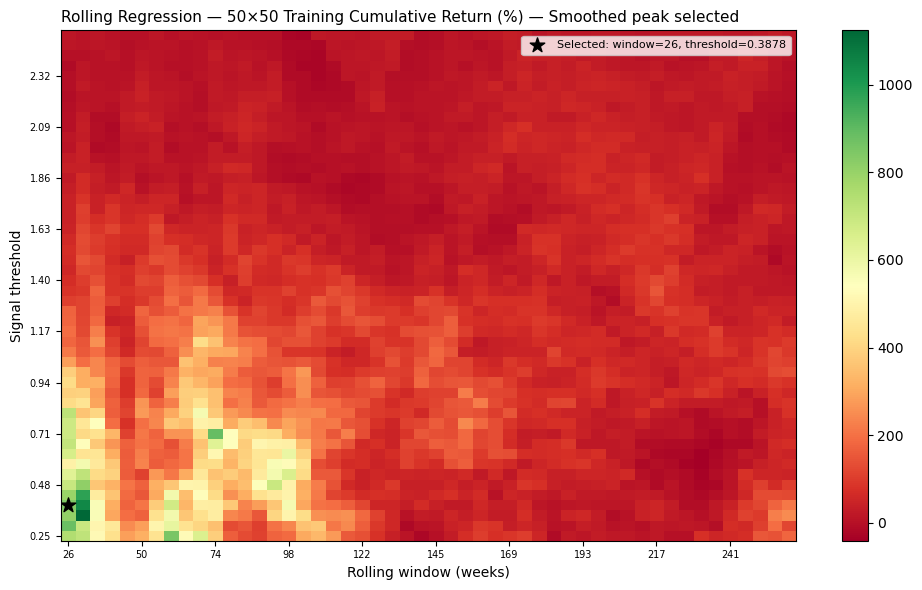
\includegraphics[width=0.80\textwidth]{figures/roll_heatmap.png}
\caption{Rolling regression hyperparameter grid on the training sample. The horizontal axis shows the trailing window length (weeks); the vertical axis shows the signal threshold (standard deviations). Colour indicates training-period cumulative return. The black star marks the neighbourhood-smoothed optimum at $W = 26$ weeks and $\tau = 0.3878$.}
\label{fig:roll_heatmap}
\end{figure}

The Kalman filter Stage~2 heatmap (Figure~\ref{fig:kf_heatmap}) illustrates the refined search surface over $q$ and $r$ at the selected threshold $\tau = 0.10$. The selected process noise $q = 2.20\times10^{-4}$ is relatively small, implying slow coefficient drift, while the low threshold allows signals to be generated frequently. The Kalman filter's selected threshold is notably lower than that of the rolling regression, suggesting a more aggressive signal regime on the training sample.

\begin{figure}[H]
\centering
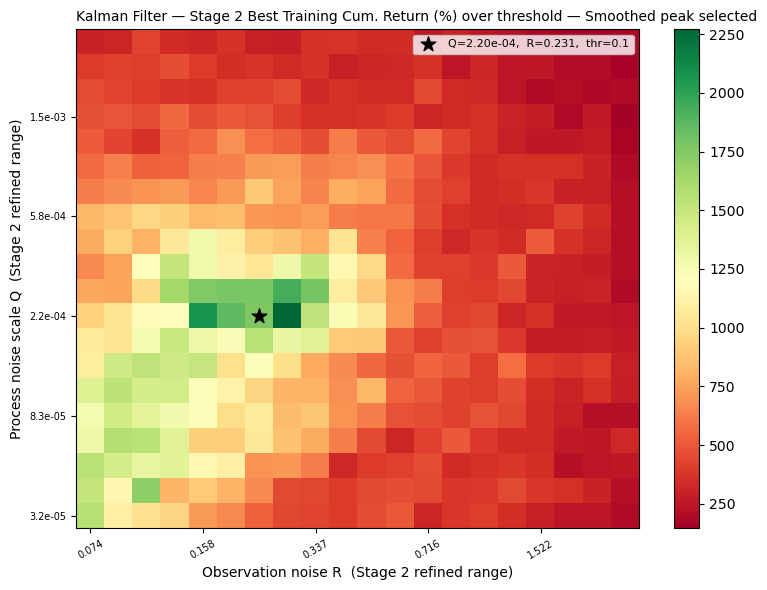
\includegraphics[width=0.72\textwidth]{figures/kf_heatmap.png}
\caption{Kalman filter Stage~2 hyperparameter grid on the training sample. Axes show the log-scaled process noise scale $q$ and observation noise $r$. The black star marks the smoothed optimum at $q = 2.20\times10^{-4}$ and $r = 0.2308$.}
\label{fig:kf_heatmap}
\end{figure}

\subsection{Training-Period Diagnostics}

Figure~\ref{fig:roll_diagnostics} shows the rolling regression training-period diagnostics: the observed S5ENRS log price alongside the model-implied fair value (top panel), the resulting gap series (middle panel), and the generated signal sequence (bottom panel). The fair value tracks the broad contour of observed price over the training period, though systematic deviations are visible—particularly around the 2008–2009 financial crisis and the 2014–2016 energy downturn. These deviations generate the signals that drive strategy returns.

\begin{figure}[H]
\centering
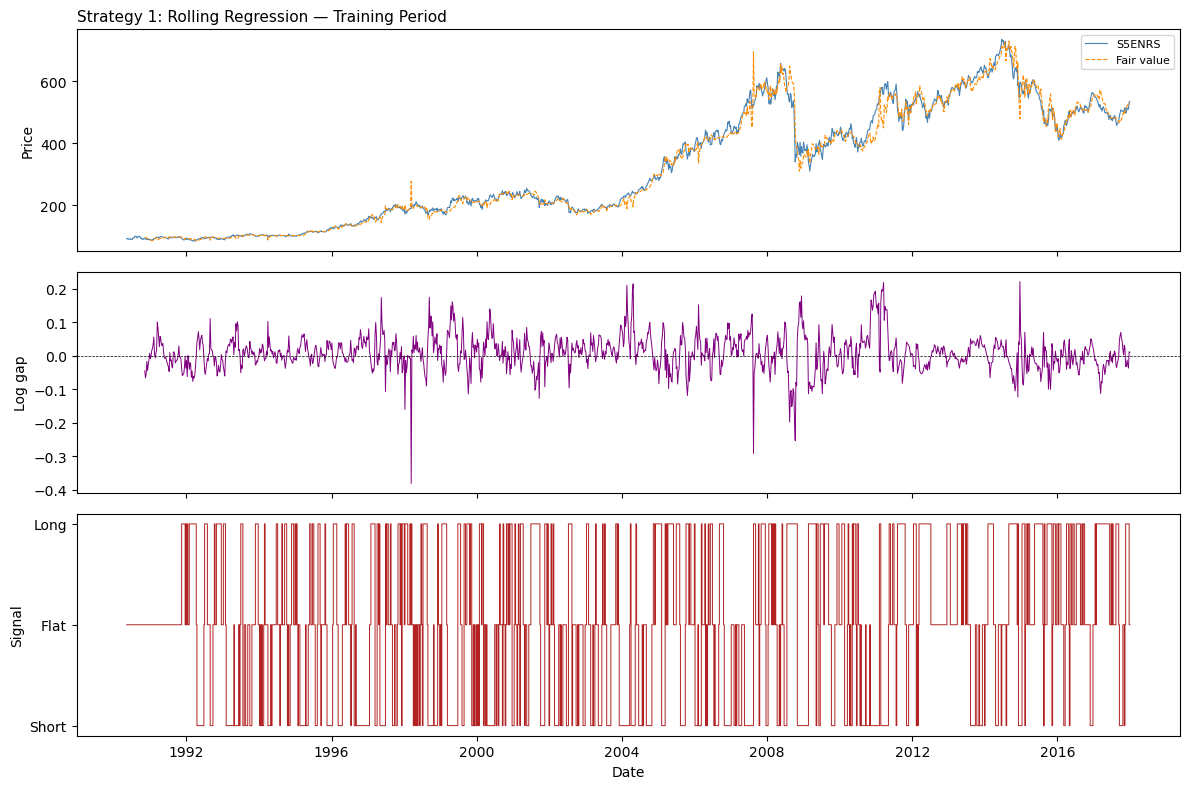
\includegraphics[width=0.95\textwidth]{figures/roll_diagnostics.png}
\caption{Rolling regression training-period diagnostics. Top: observed S5ENRS log price (blue) and model-implied fair value (orange). Middle: fair value gap in log terms. Bottom: trading signal ($+1$ = long, $0$ = flat, $-1$ = short).}
\label{fig:roll_diagnostics}
\end{figure}

\subsection{Out-of-Sample Performance}

Table~\ref{tab:performance} presents the full set of performance metrics for all four series over the out-of-sample test period from January 2018 through February 2026.

\begin{table}[H]
\centering
\caption{Out-of-Sample Performance Metrics (January 2018 – February 2026)}
\label{tab:performance}
\begin{tabular}{lrrrrrrr}
\toprule
 & Ann.\ Ret.\ (\%) & Ann.\ Vol.\ (\%) & Sharpe & Sortino & Max DD (\%) & Hit Rate (\%) & Gini \\
\midrule
Rolling Regression & 7.97 & 29.05 & 0.316 & 0.438 & $-$61.93 & 54.13 & 0.621 \\
Kalman Filter      & $-$2.89 & 28.15 & $-$0.056 & $-$0.071 & $-$59.00 & 52.12 & 0.581 \\
BnH S5ENRS         & 5.43 & 31.38 & 0.243 & 0.312 & $-$66.20 & 56.47 & 0.470 \\
S\&P 500           & 11.88 & 18.36 & 0.558 & 0.709 & $-$31.81 & 56.47 & 0.463 \\
\bottomrule
\end{tabular}

\smallskip
\footnotesize
\textit{Note:} Ann.\ Ret.\ = annualized log return; Ann.\ Vol.\ = annualized volatility; Sharpe and Sortino computed using average H15T1Y yield as risk-free rate; Max DD = maximum peak-to-trough drawdown; Hit Rate measured over active signal weeks for strategies and over all weeks for buy-and-hold; Gini = Gini coefficient of absolute weekly returns.
\end{table}

The rolling regression strategy is the clear leader among the two active strategies. It achieves an annualized return of 7.97\%, roughly 2.5 percentage points above S5ENRS buy-and-hold, and a Sharpe ratio of 0.316 versus 0.243 for the passive sector position. Its maximum drawdown of $-61.93\%$ is meaningfully smaller than the $-66.20\%$ drawdown experienced by S5ENRS buy-and-hold, consistent with the strategy's ability to move to flat or short positions during severe market dislocations.

The S\&P 500 benchmark, however, demonstrates the difficulty of matching a diversified large-cap equity index. With an annualized return of 11.88\%, a Sharpe ratio of 0.558, and a maximum drawdown of only $-31.81\%$, the benchmark substantially outperforms all three alternatives across every dimension—return, risk-adjusted return, and downside protection—over this particular eight-year window.

The Kalman filter strategy delivers a negative annualized return of $-2.89\%$ and a Sharpe ratio of $-0.056$, indicating that it destroys value out-of-sample. Despite achieving positive cumulative returns on the training data through its tuning procedure, the Kalman filter does not generalize. Its performance is consistent with a strategy that has overfitted to the training regime: it generates frequent signals under a very low threshold ($\tau = 0.10$) but those signals prove unreliable in the test period.

\subsection{Cumulative Return Comparison}

Figure~\ref{fig:cumret} plots the growth of a dollar invested in each of the four strategies from January 2018 through February 2026.

\begin{figure}[H]
\centering
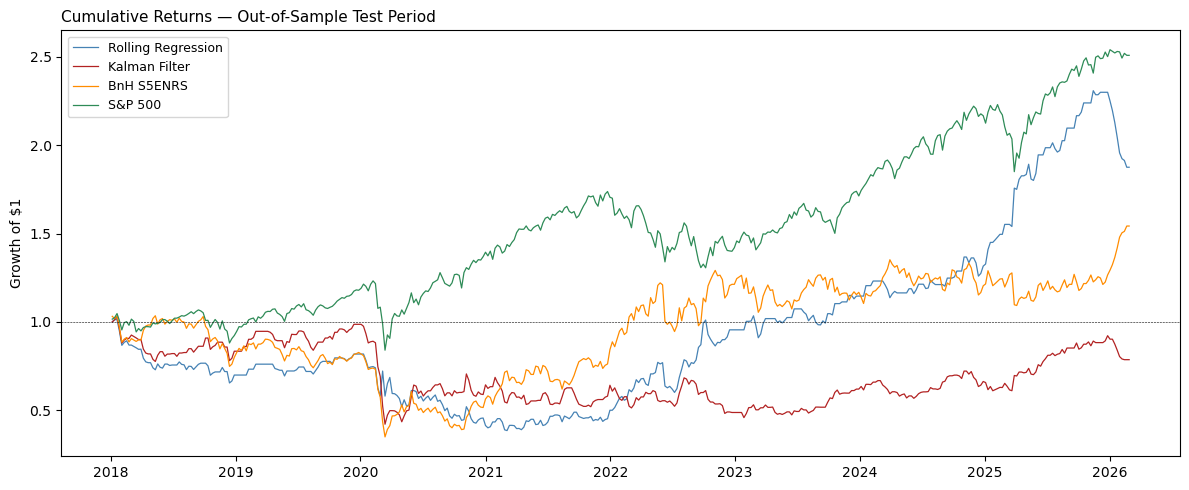
\includegraphics[width=0.95\textwidth]{figures/cumulative_returns_comparison.png}
\caption{Cumulative returns (growth of \$1) for the rolling regression strategy, Kalman filter strategy, S5ENRS buy-and-hold, and S\&P 500 benchmark over the out-of-sample test period (January 2018 – February 2026).}
\label{fig:cumret}
\end{figure}

The figure illustrates several notable patterns. The rolling regression and S5ENRS buy-and-hold track closely for extended stretches but diverge during the energy sector downturns of 2019–2020 and the post-2022 period, where the rolling regression's ability to move flat or short partially insulates it from adverse moves. The Kalman filter tracks poorly throughout the test period and drifts negative from an early stage. The S\&P 500 grows to a substantially higher level by the end of the period, compounding its return advantage into a visible gap in terminal wealth.

\subsection{Drawdown Comparison}

Figure~\ref{fig:drawdown} shows the drawdown paths for all four series.

\begin{figure}[H]
\centering
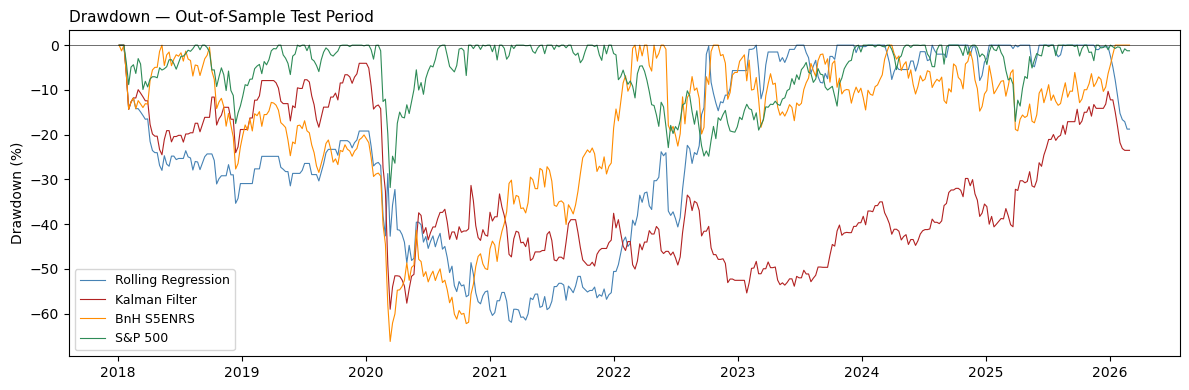
\includegraphics[width=0.95\textwidth]{figures/drawdown_comparison.png}
\caption{Drawdown paths for the rolling regression strategy, Kalman filter strategy, S5ENRS buy-and-hold, and S\&P 500 benchmark over the out-of-sample test period.}
\label{fig:drawdown}
\end{figure}

The drawdown paths confirm that S5ENRS exposure—whether passive or strategy-driven—involves substantially deeper drawdowns than the diversified S\&P 500 benchmark. The rolling regression achieves a modest drawdown reduction relative to passive S5ENRS exposure, while the Kalman filter's drawdown is nearly as large despite not generating equivalent upside. The S\&P 500's $-31.81\%$ maximum drawdown, attributable primarily to the COVID-19 shock of early 2020, appears shallow by comparison.

\subsection{Return Concentration and Hit Rates}

The Gini coefficients in Table~\ref{tab:performance} reveal that both active strategies exhibit more concentrated return profiles than the buy-and-hold benchmarks. The rolling regression Gini of 0.621 is notably higher than S5ENRS buy-and-hold (0.470) and the S\&P 500 (0.463), indicating that a disproportionate share of the strategy's cumulative return is generated in a small number of active weeks. This concentration is a feature of threshold-based signal generation: the strategy is either heavily engaged or entirely flat, leading to episodic rather than steady compounding.

Hit rates for both strategies are modestly above 50\%: 54.13\% for the rolling regression and 52.12\% for the Kalman filter over active signal weeks. These figures indicate weak but positive directional accuracy for the rolling regression, while the Kalman filter's marginal positive hit rate is insufficient to overcome its signal generation costs. Neither hit rate is evaluated for statistical significance; the sample of 426 test weeks provides limited statistical power for distinguishing signal from noise at these margins.

\subsection{Sensitivity and Robustness}

The rolling regression's selected window of 26 weeks is the shortest edge of the search grid, and its threshold of 0.3878 standard deviations sits near the low end of the candidate range. This configuration generates a high signal frequency, meaning the strategy holds a long or short position in most weeks. The concentration of training-sample performance near the short-window, low-threshold region of the grid suggests that the optimal specification is sensitive to these boundary conditions; modest changes in the selected window or threshold would alter the frequency and directionality of signals meaningfully. This sensitivity is acknowledged as a limitation of the current results.

%% ==================================================================
\section{Conclusion}
\label{sec:conclusion}
%% ==================================================================

This paper examines whether macro valuation variables can support a fundamentals-based weekly trading strategy for the S\&P 500 Energy Sector Index. Two estimation frameworks are compared: a rolling OLS regression that adapts to recent data by discarding observations outside a fixed trailing window, and a Kalman filter that allows regression coefficients to evolve as a random walk. Both strategies generate long, flat, and short signals based on deviations between observed prices and model-implied fair values, tuned on a 27.8-year training sample and evaluated out-of-sample over 8.2 years from January 2018 through February 2026.

The principal finding is that the rolling regression strategy modestly outperforms S5ENRS buy-and-hold on both an absolute and risk-adjusted basis, achieving an annualized return of 7.97\% versus 5.43\%, a higher Sharpe ratio (0.316 vs.\ 0.243), and a smaller maximum drawdown ($-61.93\%$ vs.\ $-66.20\%$). These results are encouraging in a narrow sense: they suggest that macro valuation signals derived from the Treasury yield and the broad market P/E ratio do carry some incremental predictive content for weekly energy sector returns, and that a threshold-based mean-reversion strategy can partially capture that content out-of-sample.

The caveat is equally clear. The rolling regression strategy does not approach the S\&P 500 benchmark, which returned 11.88\% annualized with a Sharpe ratio of 0.558 and far smaller realized drawdowns over the same period. The strategies studied here trade a single, relatively volatile sector index, and their performance reflects sector-specific risk that is not compensated commensurately over this particular evaluation window. Whether the rolling regression's advantage over passive sector exposure reflects a genuine, durable pricing inefficiency or a coincidence of the evaluation period cannot be resolved from a single eight-year backtest.

The Kalman filter strategy does not deliver competitive out-of-sample performance. Its $-2.89\%$ annualized return suggests that the selected hyperparameters—particularly the very low signal threshold of 0.10—reflect training-period overfitting. The Kalman filter's additional parametric flexibility appears to be a liability rather than an asset in this setting, generating frequent low-confidence signals that accumulate to negative net performance.

Several limitations bear acknowledgment. No transaction costs or market impact are modeled; energy sector ETFs typically have non-trivial bid-ask spreads, and a strategy generating frequent signals at weekly frequency would incur non-negligible implementation costs. The hyperparameters are held fixed across the entire test period; in practice, a practitioner might update them periodically, though doing so risks introducing subtle leakage. The strategy's inputs—the 1-year Treasury yield and the broad market trailing P/E—are not specific to the energy sector and may be poor proxies for the commodity-market and capex-cycle dynamics that most directly drive energy valuations. Finally, the short rolling window of 26 weeks means the model discards substantial historical context each period; its selected parameters sit near the boundary of the search grid, suggesting that the training-sample optimum may be unstable.

In sum, the rolling regression fair value gap strategy provides a modest improvement over passive S5ENRS exposure over the period studied, but falls well short of the S\&P 500 benchmark. The results are consistent with the hypothesis that macro valuation variables contain some slow-moving predictive content for energy sector returns, but they do not constitute evidence of a robust, economically large forecasting advantage.

%% ==================================================================
\section*{References}
\addcontentsline{toc}{section}{References}

\begin{description}
\item[\normalfont Federal Reserve Board (2026).] \textit{Selected Interest Rates (H.15)}.
  Board of Governors of the Federal Reserve System.
  \url{https://www.federalreserve.gov/releases/h15/}

\item[\normalfont S\&P Dow Jones Indices (2026).] \textit{S\&P 500 Index — Price, Earnings, and P/E Data}.
  S\&P Global.

\item[\normalfont Welch, G., \& Bishop, G. (1995).] An introduction to the Kalman filter.
  \textit{Technical Report TR 95-041}, University of North Carolina at Chapel Hill.

\item[\normalfont Harvey, A.C. (1990).] \textit{Forecasting, Structural Time Series Models and the Kalman Filter}.
  Cambridge University Press.

\item[\normalfont Campbell, J.Y., \& Thompson, S.B. (2008).] Predicting excess stock returns out of sample:
  Can anything beat the historical average?
  \textit{Review of Financial Studies}, 21(4), 1509–1531.
\end{description}
%% ==================================================================

\appendix

%% ==================================================================
\section{Additional Figures}
\label{app:figures}
%% ==================================================================

\subsection{Data Audit}

Figure~\ref{fig:data_audit} shows the full history of S5ENRS, the 1-year Treasury yield, and the S\&P 500 P/E ratios used in the analysis.

\begin{figure}[H]
\centering
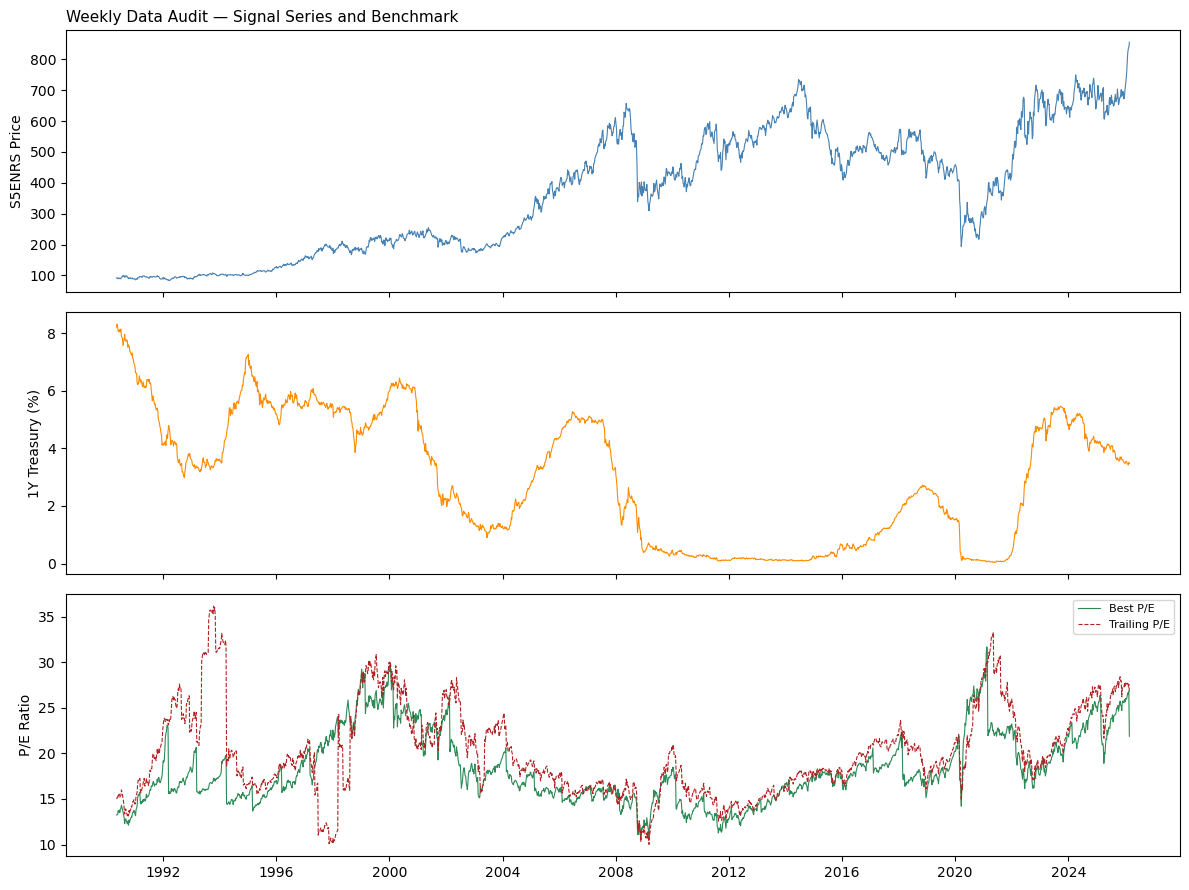
\includegraphics[width=0.95\textwidth]{figures/cell_18_fig_0.png}
\caption{Full-sample data audit. Top: S5ENRS index level. Middle: U.S.\ 1-year Treasury yield (H15T1Y). Bottom: S\&P 500 trailing P/E (SP500 PE) and forward P/E (SP500 Best PE).}
\label{fig:data_audit}
\end{figure}

\subsection{Train–Test Split}

Figure~\ref{fig:split} illustrates the S5ENRS price series with the January 5, 2018 train–test boundary marked.

\begin{figure}[H]
\centering
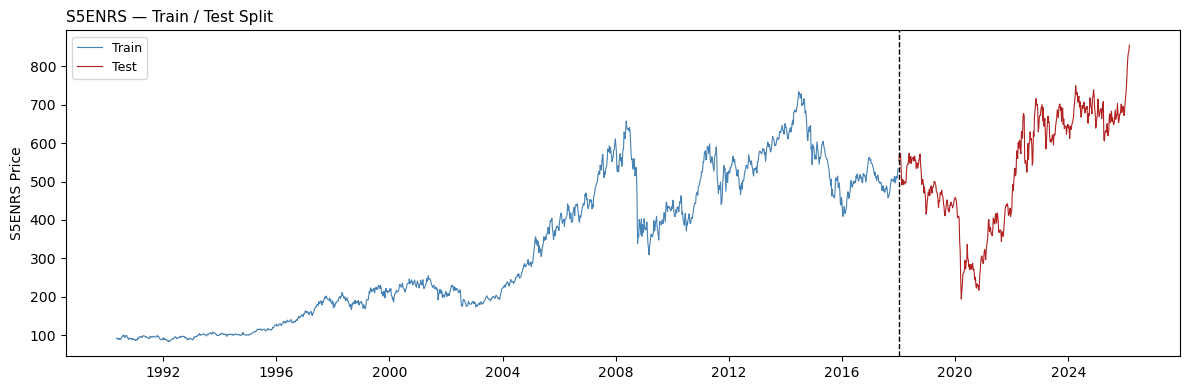
\includegraphics[width=0.95\textwidth]{figures/cell_23_fig_0.png}
\caption{S5ENRS price series with train–test split at January 5, 2018. Training period shown in blue; test period shown in red.}
\label{fig:split}
\end{figure}

\subsection{Kalman Filter Training Diagnostics}

Figure~\ref{fig:kf_diagnostics} shows the analogous training-period diagnostics for the Kalman filter strategy.

\begin{figure}[H]
\centering
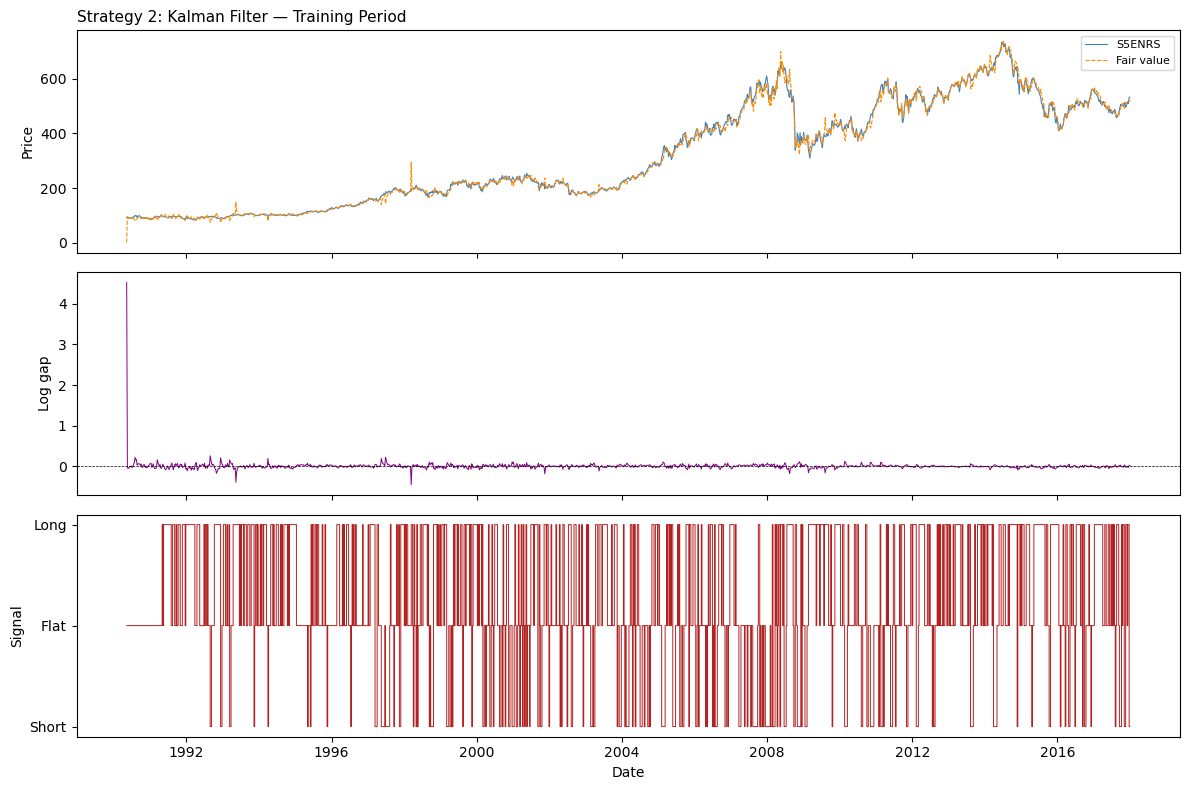
\includegraphics[width=0.95\textwidth]{figures/cell_45_fig_0.png}
\caption{Kalman filter training-period diagnostics. Top: observed S5ENRS log price (blue) and Kalman-implied fair value (orange). Middle: fair value gap. Bottom: trading signal ($+1$ = long, $0$ = flat, $-1$ = short).}
\label{fig:kf_diagnostics}
\end{figure}

\subsection{Test-Period Signal Timelines}

Figure~\ref{fig:signals_test} displays the signal series for both strategies over the test period.

\begin{figure}[H]
\centering
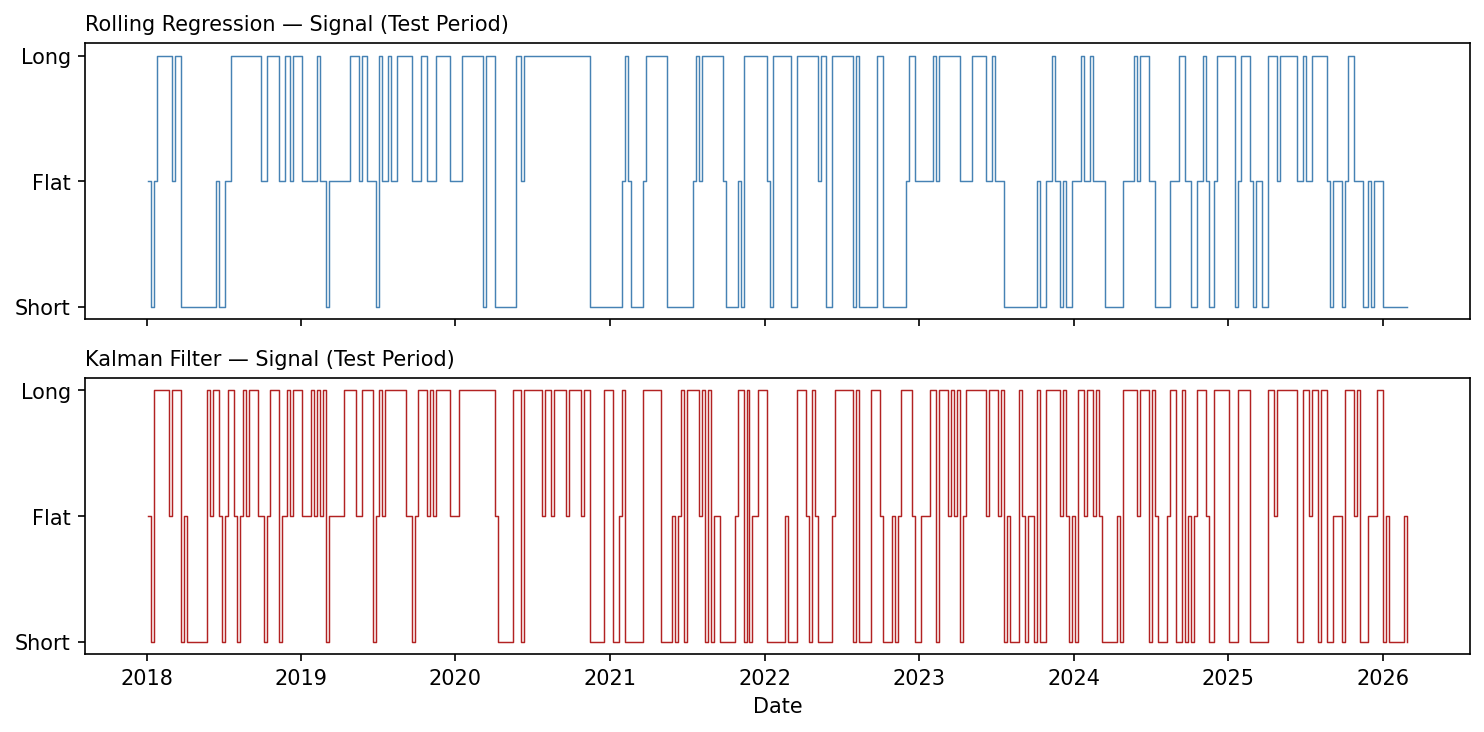
\includegraphics[width=0.95\textwidth]{figures/signals_test.png}
\caption{Test-period signals for the rolling regression (top) and Kalman filter (bottom) strategies. Steps indicate $+1$ (long), $0$ (flat), and $-1$ (short) positions for each week.}
\label{fig:signals_test}
\end{figure}

\end{document}
